\documentclass[border=4pt]{standalone}
\usepackage{fontspec}
\usepackage{amsmath}
\usepackage{unicode-math}
\setmainfont{Latin Modern Roman}
\setmathfont{Latin Modern Math}
\usepackage{pgfplots}
\usepackage{pgfplotstable}
\pgfplotsset{compat=1.18}
\usepackage{tkz-euclide}
\usetikzlibrary{arrows.meta,calc,angles,quotes,patterns,3d,backgrounds}
\definecolor{ink}{HTML}{123428}
\definecolor{asy}{HTML}{475569}
\definecolor{mint}{HTML}{86e0bd}
\tikzset{asym/.style={asy, line width=0.9pt, dash pattern=on 5pt off 3.5pt},
         guide/.style={gray!70, line width=0.6pt, densely dotted},
         dot/.style={circle, inner sep=0pt, minimum size=5pt, draw=white, line width=0.5pt},
         odot/.style={circle, inner sep=0pt, minimum size=5.5pt, fill=white, line width=1pt},
         lab/.style={font=\footnotesize, inner sep=1.5pt, text=ink}}
\begin{document}
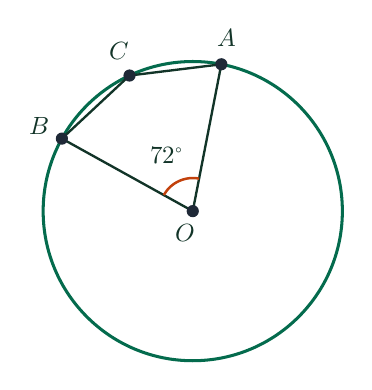
\begin{tikzpicture}
\draw[color={rgb,255:red,4;green,107;blue,77}, line width=1.1pt] (0,0) circle (1.900);
\draw[ink, line width=0.85pt] (-0.803,1.722) -- (0.363,1.865);
\draw[ink, line width=0.85pt] (-0.803,1.722) -- (-1.662,0.921);
\draw[ink, line width=0.85pt] (0.000,0.000) -- (0.363,1.865);
\draw[ink, line width=0.85pt] (0.000,0.000) -- (-1.662,0.921);
\draw[color={rgb,255:red,194;green,65;blue,12}, line width=0.9pt] (0.080,0.412) -- (0.054,0.417) -- (0.028,0.419) -- (0.001,0.420) -- (-0.025,0.419) -- (-0.051,0.417) -- (-0.077,0.413) -- (-0.103,0.407) -- (-0.128,0.400) -- (-0.153,0.391) -- (-0.177,0.381) -- (-0.201,0.369) -- (-0.224,0.355) -- (-0.246,0.341) -- (-0.267,0.325) -- (-0.286,0.307) -- (-0.305,0.289) -- (-0.323,0.269) -- (-0.339,0.248) -- (-0.354,0.226) -- (-0.367,0.204);
\node[font=\small, text=ink, inner sep=0.5pt, fill=white] at (-0.330,0.707) {$72^\circ$};
\fill[color={rgb,255:red,31;green,41;blue,55}] (0.363,1.865) circle (2.2pt);
\fill[color={rgb,255:red,31;green,41;blue,55}] (-1.662,0.921) circle (2.2pt);
\fill[color={rgb,255:red,31;green,41;blue,55}] (-0.803,1.722) circle (2.2pt);
\fill[color={rgb,255:red,31;green,41;blue,55}] (0.000,0.000) circle (2.2pt);
\node[font=\small, text=ink, inner sep=0.5pt] at (0.427,2.199) {$A$};
\node[font=\small, text=ink, inner sep=0.5pt] at (-1.959,1.086) {$B$};
\node[font=\small, text=ink, inner sep=0.5pt] at (-0.947,2.030) {$C$};
\node[font=\small, text=ink, inner sep=0.5pt] at (-0.103,-0.282) {$O$};
\end{tikzpicture}
\end{document}
